\chapter{Organisational Mission and Goals}
\label{cap:visiongoals}

%   Savas
\section{Mission}

The Bank's cuyrrent state is composed by various levels divided into divisions, departments and operational units, as well represented into the organization organigram in Figure~\ref{fig:organization_organigram}.
The recent acquisition of overseas banks has positioned the Bank at an international level, changing its requirements and creating new opportunities to expand and enhance the services provided. 
To ensure the realization of the vision, Information Technology (IT) Department cover a strategic role, by adopting the structure of a \textbf{``Shared Service Center''} thus to ensure that business services remains reliable, secure and efficient; while providing high-performance, high-quality, and cost-effective services both internally than externally to the organization.

\begin{figure}[h]
    \centering
    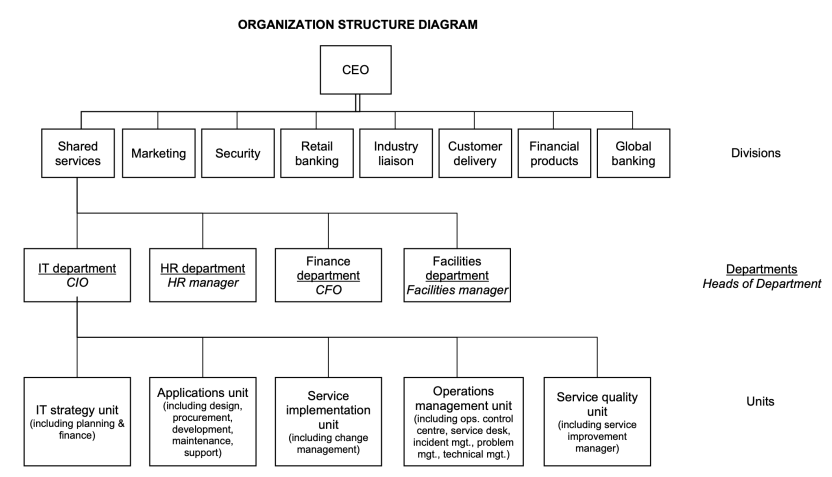
\includegraphics[width=0.8\textwidth]{images/organization_organigram.png}
    \caption{Organization Organigram}
    \label{fig:organization_organigram}
\end{figure}


%   Still working on it its gonna grow

\section{Goals}

% • Focus on value 
% • Start where you are 
% • Progress iteratively with feedback 
% • Collaborate and promote visibility  
% • Think and work holistically
% • Keep it simple and practical 
% • Optimize and automate 



% This strategic transformation is driven by the objective of increasing value for both the organization and its customers by offering innovative, reliable, and internationally integrated banking services \textit{(focus on value)}.

% This centralized approach enables better coordination, reducing duplicated activities and improves service consistency through the organization. The first step is to analyze what logic and process the banks acquired have adopted , and to analyze the current IT environment, so identifying existing strengths and weaknesses.


To support the Mission of the company, the primary goal of the IT Department is to implement a ``Performance-Based Management'' approach. Through this model, organizational performance is continuously monitored via measurable Key Performance Indicators, which provide objective information for decision-making \textit{(progress iteratively with feedback)}. Decisions based on measurable data, rather than subjective opinions enable management to identify weaknesses and monitor progress toward strategic objectives; thus to evaluate the effectiveness of implemented improvements and continuously enhance service quality.

To achieve these strategic objectives, the Bank has identified three Critical Success Factors (CSFs)\gls{csf}, representing the key areas that require enforcement and attention.

\begin{itemize}
    \item \textbf{Customer Partnership} represnets the first Critical Success Factor. As the Bank expands its international presence and strengthens collaborations with external financial institutions and independent financial advisors, establishing strong relationships with customers and business partners becomes essential \textit{(collaborate and promote visibility)}. The IT Department therefore works closely with business units to actively involve stakeholders throughout the service lifecycle. Through continuous communication, customer feedback and satisfaction surveys, IT can better understand business needs and deliver services that enrich value for customers while supporting the Bank's strategic business.
    As indicated by the corporation and business strategy by the bank:
    \begin{itemize}
        \item In the bank's HQ country, to have as a customer base 10\% of the retail banking market (currently 7~\%)
        \item To increase income from internet banking by 70%
        \item  To increase the income from customers living outside the HQ country by 50\%
        \item To achieve a 5\% increase in corporate profit.
    \end{itemize}

    \item The second Critical Success Factor is \textbf{Process Factory}. The Bank aims to standardize current IT processes, technologies, and operational procedures across all acquired organizations and various departments \textit{(start where you are)}. Standardization reduces complexity, minimizes waste, simplifies maintenance activities and improves service consistency. \\
    Furthermore, standardized processes facilitate the integration of different IT environments and create a clearer workflow of the process, enabiling a more efficeint management of services on an international scale \textit{(keep it simple and practical)}. 
    This objective is particularly important and fragile, since the Bank while maintaining high levels of service quality in multiple countires must ensure different regulations compliance of various nature: Political, Economical, Social, Technological, Environmental and Legal (PESTLE). 
    
    
    \item The third Critical Success Factor is \textbf{Continuous Improvement}. The Bank recognizes that delivering high-quality IT services requires continuous measurement, evaluation and optimization toward to improve the value provided \textit{(focus on value)}. \\
    This initiative must be done by collecting and analyzing performance data generated through KPIs~\gls{kpi}; then the corporation can identify opportunities for improvement and monitor potential risks.
    Overral through incremental improvements, regular feedback, and continuous evaluation of results, the organization can steadily increase the value delivered to customers while optimizing both services and internal resources \textit{(think and work holistically)}.
\end{itemize}

To verify whether these Critical Success Factors are being achieved, the Bank has defined a KPI \gls{kpi} tree composed of six Key Performance Indicators.


Together, these KPIs \gls{kpi} provide a balanced overview of service quality, operational efficiency, customer satisfaction and financial performance.
By continuously monitoring these indicators, and where possible, automating the collection and analysis of performances \textit{(optimize and automate)}, the IT Department can ensure that its activities be aligned with overall business strategy.
Furthermore, KPI \gls{kpi} monitoring supports Service Level Management, enabling the organization to identify areas that require corrective actions and ensure that the service provided accomplish the customer expectations. Moreover, all these procedures ensure the continuous progress toward its strategic objectives \textit{(keep momentum going)}.


% \begin{figure}[h]
%     \centering
%     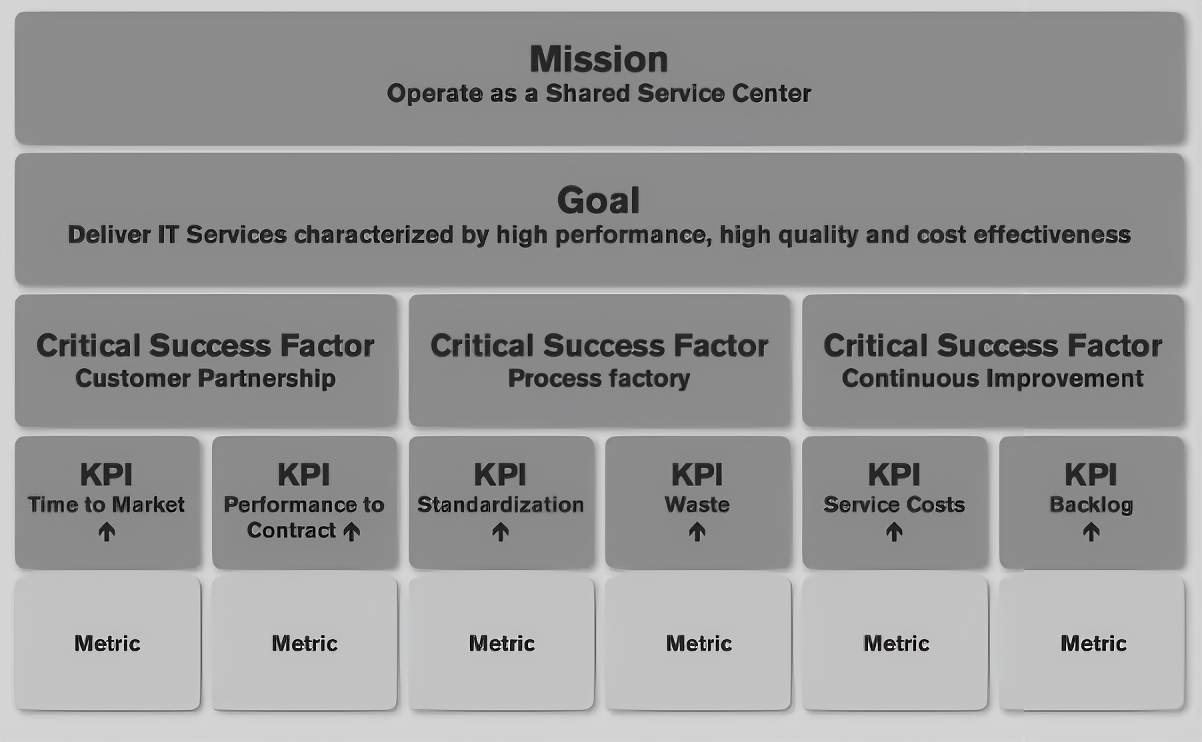
\includegraphics[width=0.8\textwidth]{images/vision.png}
%     \caption{what to do}
%     \label{fig:whattodo}
% \end{figure}
